%!TEX root = ../thesis.tex
\chapter{Conclusions}
\label{conclusions}

\section{Improvement and future implementations}
%
%	Now that I have explained how the project was implemented
%
%Now that all the work has been explained, let's see how it turned out and what can be done to improve it in the future

\section{Final Gantt diagram}
%	come si discosta da quello iniziale\\
%	cosa ha causato questo discostamento\\
%	ho pianificato male
%	
	\hl{MOVE IMAGE IN APPENDIX}
	\begin{figure}[H]
		\centering
		\makebox[\textwidth][c]{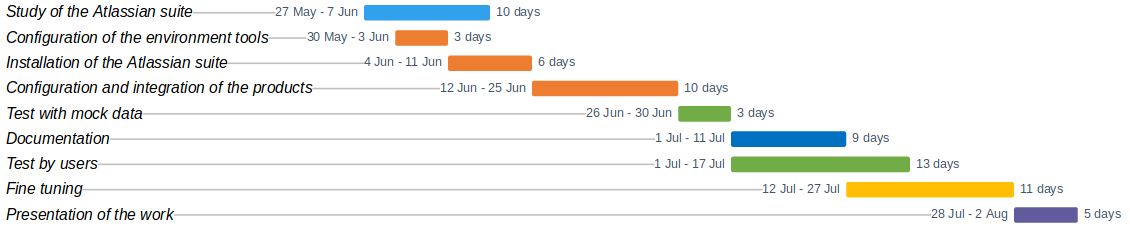
\includegraphics[width=1.15\textwidth]{resources/revised_gantt}}%
%		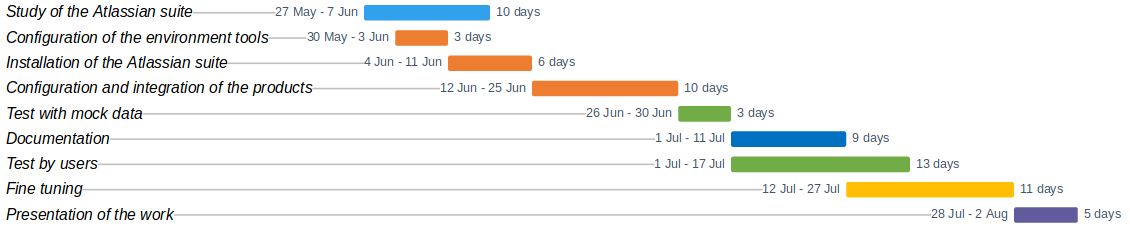
\includegraphics[width=\textwidth]{resources/revised_gantt}\\
		\caption{Dilbert on Agile Programming}
	\end{figure}
	
\section{Objectives achievement}

\section{What I have learned}
%	principalmente il way of working aziendale\\
%	come funzionano questi tool\\
%	il loro scopo di "ordinare" un'azienda

\section{Personal considerations}
%	in un'azienda in crescita è molto utile darsi dei paletti\\
%	in athonet funzionerà una cosa del genere?  software monolitico / complesso (service oriented architecture)\\
%	sta funzionando questo tool adesso per il breve tempo che l'ho visto io in produzione?
%	valore aggiunto all'azienda, cosa vede il cliente

%	Quanto i corsi universitari mi abbiano preparato ed aiutato ad affrontare uno stage di questo tipo